\documentclass[11pt, oneside]{article} 
\usepackage{geometry}
\geometry{letterpaper} 
\usepackage{graphicx}
	
\usepackage{amssymb}
\usepackage{amsmath}
\usepackage{parskip}
\usepackage{color}
\usepackage{hyperref}

\graphicspath{{/Users/telliott/Github/calculus_book/png/}}
% \begin{center} 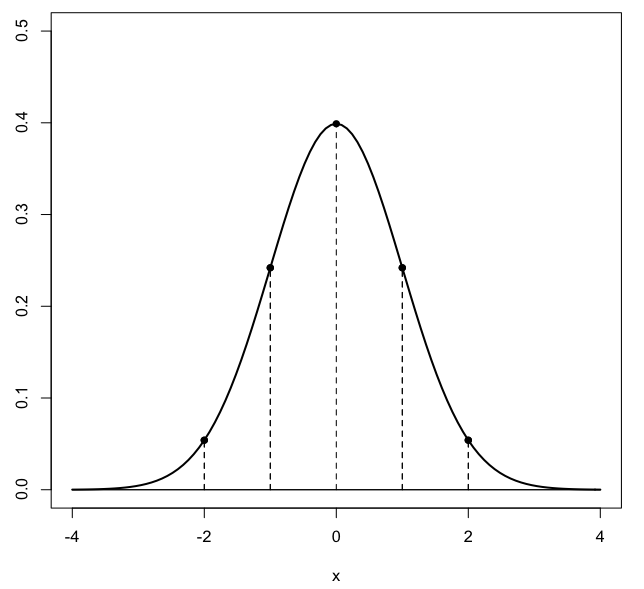
\includegraphics [scale=0.4] {gauss3.png} \end{center}

\title{Analytic geometry}
\date{}

\begin{document}
\maketitle
\Large

It is difficult today to put ourselves in the place of those who tried to reason about mathematics through the ages.  

The Greeks lacked algebra, and although the Romans worked with numbers they did not have decimal notation.  The concept of $0$ came much later (from India), and even in the Middle Ages there was as yet no such thing as the equals sign $=$, which dates from 1557.

\url{https://en.wikipedia.org/wiki/Table_of_mathematical_symbols_by_introduction_date}

The invention of analytic geometry is often ascribed solely to Descartes, but Fermat also had his own version.  There are two fundamental ideas.
\begin{center} 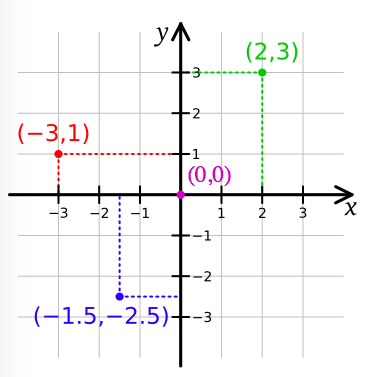
\includegraphics [scale=0.45] {coordinates.png} \end{center}

The first is to orient two number lines on a piece of paper, at right angles, and then consider pairs of numbers $(x,y)$ in the 2D plane.  Such pairs or tuples are called points.

Descartes published this idea in 1637.  The presentation would be difficult to recognize as our current system, but the germ is there:  axes where the position of a variable could be marked.  Only the positive numbers would be shown, and the axes not necessarily perpendicular.  As to the proofs, here is wikipedia on the subject:

\begin{quote} \textcolor{blue}{His exposition style was far from clear, the material was not arranged in a systematic manner and he generally only gave indications of proofs, leaving many of the details to the reader.  His attitude toward writing is indicated by statements such as "I did not undertake to say everything," or "It already wearies me to write so much about it," that occur frequently. In conclusion, Descartes justifies his omissions and obscurities with the remark that much was deliberately omitted "in order to give others the pleasure of discovering [it] for themselves."}
\end{quote}

The second idea of analytic geometry is to plot all the points that satisfy some mathematic relationship between $x$ and $y$, for example the parabola $y=x^2$.  

To do this, pick a few values of $x$ and calculate the corresponding values of $y$.  For example:  $(0,0), (\pm 1,1), (\pm 2, 4), \dots$.  Plot these points, and then finally, sketch the graph of the curve, without actually trying to plot \emph{all} of the individual points (of which there is an infinite number).  We make the assumption here that the function being plotted is continuous, so that the sketch of a curve between two points that are close enough together will be fairly smooth and if the $x$-values are close to the plotted $x$, the corresponding $y$-values will not be not too different from the plotted $y$.

\subsection*{point}
A point is simply an ordered pair $(x,y)$ such as $(1,3)$.  Often points have integer components, but they don't have to be.

\subsection*{distance formula}
The $x$- and $y$-axes are perpendicular to one another (a fancy word for that is \emph{orthogonal}).  

Suppose we pick two particular points $(s,t)$ and $(u,v)$, plot them on a graph, and then draw the line that connects them.  Recall Euclid's first two postulates:

$\circ$  A straight line segment can be drawn joining any two points.

$\circ$   Any straight line segment can be extended indefinitely in a straight line.

The distance between the two points is given by the Pythagorean formula, where $\Delta x$ is the change in $x$ and $\Delta y$ is the change in $y$:
\[ d = \sqrt{\Delta x^2 + \Delta y^2} \]
It is often easier to use the squared distance and avoid the square root:
\[ d^2 = \Delta x^2 + \Delta y^2 \]
\[ = (s-u)^2 + (t-v)^2 \]
Switching the order of $(s,t)$ and $(u,v)$ doesn't change the result.

\subsection*{formulas for a line}
 
Now we want to derive an equation that describes (is valid for) all the points or pairs of values $(x,y)$ on this line.  A general approach is to say that the line has some slope $m$, which is defined as $\Delta y$, divided $\Delta x$:
\[ m = \frac{\Delta y}{\Delta x} = \frac{y-y'}{x-x'} \]

This is called the \emph{point-slope equation}.  For any two particular points $(s,t)$ and $(u,v)$ one can plot a line between them.  The slope is
\[ m = \frac{s - u}{t - v} \]

One can write the two points in either order, with the same result since:
\[ \frac{s - u}{t - v} = \frac{u - s}{v - t} \]

Depending on the details, the value of $m$ might be zero, for a horizontal line, where all the values of $y$ are the same (which happens when $s = u$).  Or it might be undefined, for a vertical line, where all the values of $x$ are identical ($t = v$).  

In most cases, however, $m \ne 0$ and $m \in (-\infty, \infty)$.  That is, $m$ is usually non-zero and not infinite.

Except in the case of the vertical line, we can write
\[ y = mx + y_0 \]
for any point $(x,y)$ on a given line, where $y_0$ is the $y$-intercept, the value of $y$ obtained when $x = 0$.

[ The choice of $b$ for the $y$-intercept is the usual notation, but it conflicts with another $b$ that we will see in a minute. ]

$y = mx + y_0$ is the \emph{slope-intercept equation} of the line.

The equation of a line is determined by both the slope and one point on the line, for example the $y$-intercept.  One can draw a whole family of parallel lines with the same slope and different $y$-intercepts.  Here are three lines $y = 2x + y_0$ for $y_0 = \{ 0, 1, 2 \}$.

\begin{center} 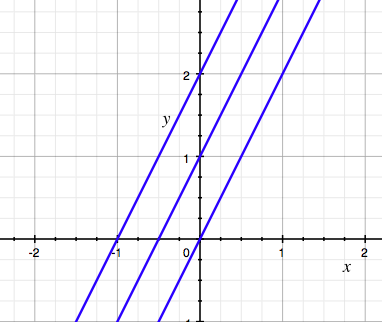
\includegraphics [scale=0.4] {line_family.png} \end{center}

The value of $x$ corresponding to $y = 0$ is the $x$ intercept
\[ x_0 = -\frac{y_0}{m} \]

The point-slope equation is easily derived from the second one.  Suppose we have $y = mx + y_0$:

Plugging in for specific points $(s,t)$ and $(u,v)$ we have
\[ t = ms + y_0 \]
\[ v = mu + y_0 \]
Subtracting:
\[ v - t = m(u - s) \]
which rearranges to give the desired result.

\subsection*{intersections}
Often one has two lines (or curves) and we want to find the point(s) that lie on both.  We might have
\[ y = 2x - 1 \]
\[ y = -x + 8 \]
Substitute from the second into the first:
\[ 2x - 1 = -x + 8 \]
\[ 3x = 9 \]
\[ x = 3 \]
From the first equation, $y = 5$, and we check that $x = 3, y = 5$ solves the second equation as well.

\subsection*{orthogonality}
If two lines cross each other at right angles we say they are \emph{orthogonal}.  In that case the slopes have a special relationship.  Their product is equal to $-1$.

\begin{center} 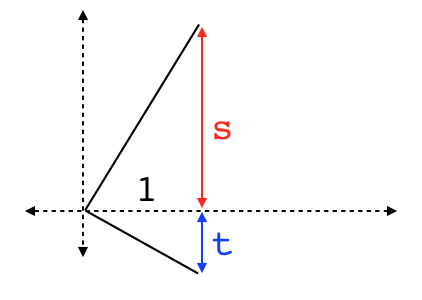
\includegraphics [scale=0.4] {slopes_ortho.png} \end{center}

Here is a simple proof.  Draw the two lines going through the origin, forming a right angle there.  The first has slope $s$, so it goes through the point $(1,s)$, the second goes through $(1, t)$.  

Recall from the chapter on the Pythagorean theorem that the altitude squared is equal to the product of the two pieces of the base.  Here:
\[ 1^2 = 1 = st \]
These are the lengths, i.e. the absolute values of the slopes.  Thus $ |s| = 1/|t|$.  But   

Clearly the sign of $t$ is negative.  So we arrive at
\[ s \cdot (-t) = 1 \]
\[ m_1 = - \frac{1}{m_2} \]

We'll see a natural easy proof of this once we look at trigonometry.  Here is a hint:

\begin{center} 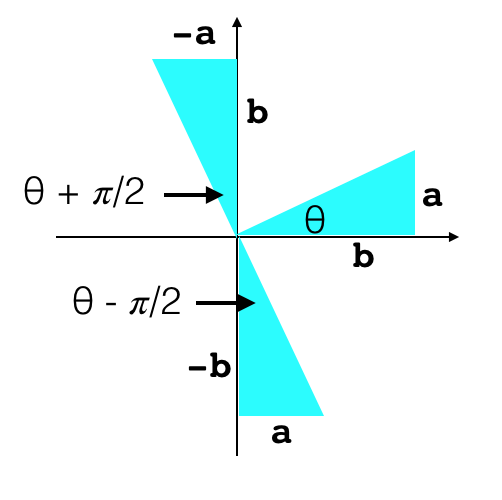
\includegraphics [scale=0.4] {rotation.png} \end{center}

\subsection*{formula for a circle}

A circle can be defined as all the points at the same distance from a central point, let us label that point $(h,k)$.  The distance from the points to the center is the radius, denoted $r$.

Using the Pythagorean theorem, we can calculate the square of the distance from the origin as
\[ r^2 = (x - h)^2 + (y - k)^2 \]

The simplest circles are those whose central point is the origin of the coordinate system.  In that case the equation  simplifies to 
\[ r^2 = x^2 + y^2 \]
Usually, we know the value of $r$ and we want to write an equation for $y$ in terms of $x$.  Then
\[ y^2 = r^2 - x^2 \]
\[ y = \sqrt{r^2 - x^2} \]

\subsection*{formula for a parabola}

A general formula for a parabola with its vertex at the point $(h,k)$ is
\[ y - k = a(x - h)^2 \]

where $a$ is called the shape factor.  It governs how steeply the curve rises (and by its sign, in which direction it opens).

Multiplying out:
\[ y - k = a(x^2 - 2xh + h^2) \]
\[ y = ax^2 - 2ah x + ah^2 + k \]

In this form the cofactors are usually simplified as
\[ y = ax^2 + bx + c \]

where
\[ b = -2ah; \ \ \ \ c = ah^2 + k \]

If the equation is given in the second form then we can find:
\[ h = -\frac{b}{2a} \]
\[ k = c - ah^2 = c - \frac{b^2}{4a} \]

Probably the most common thing we're asked to do with a quadratic equation like this is to find the roots, the values of $x$ for which $y=0$ is a solution.  These are the points where the graph of the curve crosses the $x$-axis.  (It may not do so, it is possible to have 0, 1 or 2 roots).

\begin{center} 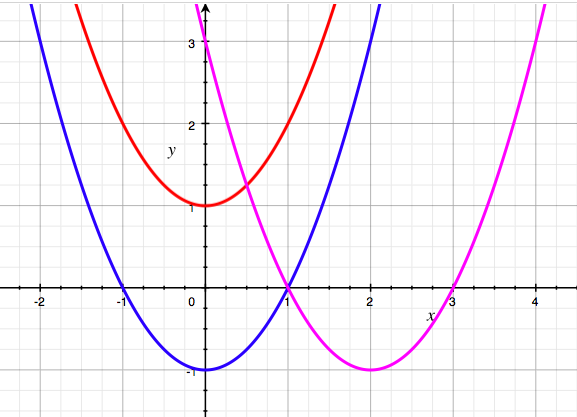
\includegraphics [scale=0.4] {para7.png} \end{center}
In the figure, the red curve does not cross the $y$-axis.  Its equation is $y = x^2 + 1$, and there are no solutions, no values of $x$ that solve the equation when $y = 0$.
\[ 0 = x^2 + 1 \]
\[ x^2 = - 1 \]

To find the roots of
\[ ax^2 + bx + c = 0 \]
We can guess solutions by trying to factor into a form like:
\[ (x - s)(x - t) = 0 \]

but roots do not have to be integers (or even rational).  An arguably more productive and certainly more general approach is the process of \emph{completing the square}.  

First, multiply through by $1/a$ and rearrange:
\[ x^2 + \frac{b}{a} x = - \frac{c}{a} \]

The key insight is to recognize that if we add $(b/2a)^2$ to both sides, the left-hand side will become a perfect square:
\[ x^2 + \frac{b}{a} x + (\frac{b}{2a})^2 = -\frac{c}{a} + (\frac{b}{2a})^2 \]
\[ (x + \frac{b}{2a})^2 = -\frac{c}{a} + (\frac{b}{2a})^2 \]
\[ x + \frac{b}{2a} = \pm \sqrt{-\frac{c}{a} + (\frac{b}{2a})^2} \]

Multiplying top and bottom of the first term under the square root gives a common factor:
\[ x + \frac{b}{2a} = \pm \sqrt{-\frac{4ac}{4a^2} + (\frac{b}{2a})^2} \]
which can come out of the square root and then matches what's in the second term on the left-hand side:
\[ x + \frac{b}{2a} = \pm \frac{\sqrt{-4ac + b^2}}{2a} \]
which we rearrange slightly to give the standard \emph{quadratic formula}:
\[ x = \frac{-b \pm \sqrt{b^2 - 4ac}}{2a} \]

\subsection*{focus and directrix}
There is also a classic geometric definition of the parabola.  

Based on what we said above, we can transform any parabola of the form $y = ax^2 + bx + c$ into a $(y - k) = a(x - h)^2$.  If we're interested in the shape of the parabola and don't care about its absolute location, then without loss of generality, we can translate any parabola to the origin of coordinates, with equation $y = ax^2$, so let us just work with that.

Now, pick a point on the $y$-axis a distance $p$ up from the origin, colored magenta in the figure.  This point is called the focus.

Then draw a line parallel to the $x$-axis which intersects the $y$-axis the same distance $p$ below the origin.  This line is called the directrix.  It is colored red and is dashed.

\begin{center} 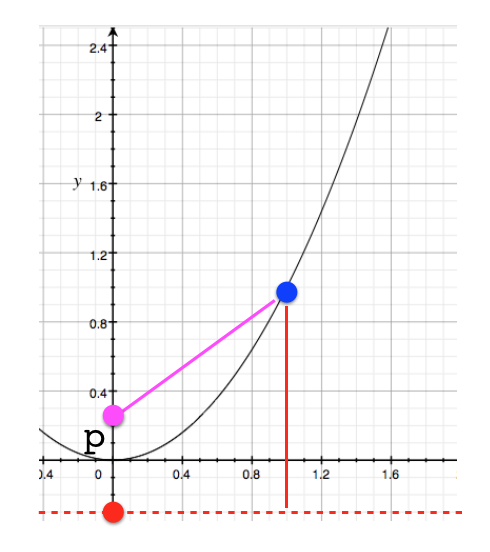
\includegraphics [scale=0.5] {para16.png} \end{center}
The parabola consists of all those points whose distance to the focus is equal to the vertical distance to the directrix.

Pick an arbitrary point on the parabola (in blue), with coordinates $(x, ax^2)$.  The squared distance to the focus (magenta) is 
\[ x^2 + (ax^2 - p)^2 \]
where $\Delta x$ is just equal to $x$ and $\Delta y$ is equal to $y - p$, with $y = ax^2$.

The squared distance to the directrix (red) is  $(ax^2 + p)^2$.  

For the correct choice of $p$ these distances will be equal:
\[ x^2 + (ax^2 - p)^2 = (ax^2 + p)^2 \]

We have $(m-n)^2$ on the left-hand side and $(m+n)^2$ on the right-hand side, so the result will have $4mn$ on the right hand side:
\[ x^2 = 4apx^2 \]

Divide by $x^2$
\[ 1 = 4ap \]
\[ p = \frac{1}{4a} \]

The shape factor $a$ determines the distance of the focus from the origin, we label that distance as $p$.  The equation of the directrix is $y = -p$.

\subsection*{slope of the tangent}
It will turn out that the slope of the tangent to $y=ax^2$ at any fixed point $x$ is equal to $2ax$. 

This is literally the first result from differential calculus, but we will also see a way to find it using analytical geometry in the next chapter, as well as a vector approach later on.

Thus, the equation of a line passing through the point $(x,ax^2)$ with the given slope is
\[ y' - ax^2 = 2ax(x' - x) \]
where $(x',y')$ is any other point on the line.

What \emph{that} means is that the $x$-intercept $x_0$ of the tangent line is:
\[ - ax^2 = 2ax x_0 - 2ax^2 \]
\[ ax^2 = 2ax x_0 \]
\[ x = 2x_0 \]
\[ x_0 = \frac{1}{2} x \]

The tangent line passes through the $x$ axis halfway back toward the origin.
\begin{center} 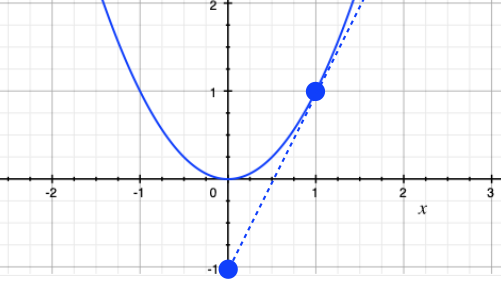
\includegraphics [scale=0.4] {para17.png} \end{center}

And what \emph{that} means is that the $y$-intercept is symmetrical with the original point (as far below the $x$-axis as the point is above it). Here's the algebra:
\[ y_0 - ax^2 = 2ax(0 - x) \]
\[ y_0 = -ax^2 \]

And then finally, if the point on the parabola is $P$, the focus $F$, the intersection with the directrix $D$, and the $y$-intercept $I$
\begin{center} 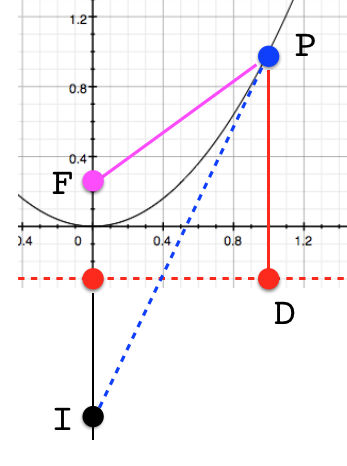
\includegraphics [scale=0.4] {para18.png} \end{center}
the quadrilateral $FPDI$ is a regular parallelogram with all four equal sides, and its long diagonal (the tangent line) makes equal angles with $FP$ and $PD$.

And what \emph{that} means is that if $PD$ is extended vertically, the angle it makes with the tangent line is equal to the angle between $FP$ and the tangent line, so that for example, all vertical light rays entering a parabola will reflect and then come together at the focus.




\end{document}